% Reporte académico de diseño e implementación de Music Database.
% Compilar con: xelatex -interaction=nonstopmode Reporte_Music_Database.tex (dos veces)
% Material de apoyo: assets/search.png, assets/library.png, assets/songform.png.
\documentclass[11pt,a4paper,oneside]{article}
\usepackage[spanish,es-noshorthands]{babel}
\usepackage{fontspec}
\setmainfont{Liberation Serif}
\setsansfont{Liberation Sans}
\setmonofont[Scale=0.86]{DejaVu Sans Mono}
\usepackage{geometry}
\geometry{top=2.35cm,bottom=2.25cm,left=2.5cm,right=2.5cm}
\usepackage{microtype}
\usepackage[table]{xcolor}
\usepackage{booktabs,tabularx,longtable,array}
\usepackage{enumitem}
\usepackage{tikz}
\usetikzlibrary{arrows.meta,positioning,shapes.geometric,fit,backgrounds,calc}
\usepackage{adjustbox}
\usepackage{graphicx}
\usepackage{float}
\usepackage{caption}
\usepackage{tcolorbox}
\tcbuselibrary{skins,breakable}
\usepackage{fancyhdr,lastpage}
\usepackage{titlesec}
\usepackage{hyperref}
\usepackage{listings}
\usepackage{setspace}
\usepackage{needspace}
\definecolor{navy}{HTML}{14243A}
\definecolor{ink}{HTML}{263748}
\definecolor{green}{HTML}{119A70}
\definecolor{pale}{HTML}{E8F5F0}
\definecolor{sky}{HTML}{EAF0F6}
\definecolor{grayline}{HTML}{CCD7DF}
\definecolor{muted}{HTML}{617180}
\definecolor{warm}{HTML}{FFF3E8}
\color{ink}
\hypersetup{colorlinks=true,linkcolor=navy,urlcolor=green,pdftitle={Music Database: reporte de diseño e integración},pdfauthor={Proyecto académico de Modelado y Programacion},pdfsubject={Arquitectura MVC, SQLite, TagLibSharp, Avalonia UI y MusicMiner}}
\setlength{\parindent}{0pt}
\setlength{\parskip}{6.5pt}
\setlength{\emergencystretch}{2em}
\setlist[itemize]{leftmargin=1.5em,itemsep=2pt,topsep=3pt}
\setlist[enumerate]{leftmargin=1.55em,itemsep=2pt,topsep=3pt}
\titleformat{\section}{\Large\bfseries\sffamily\color{navy}}{\thesection.}{0.65em}{}
\titleformat{\subsection}{\large\bfseries\sffamily\color{navy}}{\thesubsection}{0.7em}{}
\titleformat{\subsubsection}{\normalsize\bfseries\sffamily\color{ink}}{\thesubsubsection}{0.7em}{}
\titlespacing*{\section}{0pt}{20pt}{8pt}
\titlespacing*{\subsection}{0pt}{12pt}{5pt}
\pagestyle{fancy}
\fancyhf{}
\fancyhead[L]{\sffamily\footnotesize\color{muted} MUSIC DATABASE}
\fancyhead[R]{\sffamily\footnotesize\color{muted} REPORTE TÉCNICO}
\fancyfoot[L]{\sffamily\footnotesize\color{muted} Noviembre de 2026}
\fancyfoot[R]{\sffamily\footnotesize\color{muted} \thepage\ de \pageref{LastPage}}
\renewcommand{\headrulewidth}{0.35pt}
\renewcommand{\footrulewidth}{0pt}
\setlength{\headheight}{15pt}
\captionsetup{font=small,labelfont={bf,sf},textfont=it,justification=centering}
\newtcolorbox{notabox}[1][]{enhanced,breakable,boxrule=0.6pt,colframe=grayline,colback=sky,arc=2mm,left=3mm,right=3mm,top=2mm,bottom=2mm,#1}
\newtcolorbox{hallazgobox}[1][]{enhanced,breakable,boxrule=0.6pt,colframe=green,colback=pale,arc=2mm,left=3mm,right=3mm,top=2mm,bottom=2mm,#1}
\newcommand{\file}[1]{\texttt{\detokenize{#1}}}
\newcommand{\code}[1]{\texttt{\detokenize{#1}}}
\newcommand{\R}{\textsf{MusicMiner}}
\newcommand{\A}{\textsf{MusicApp}}
\lstdefinestyle{commands}{basicstyle=\ttfamily\footnotesize,frame=single,framerule=.4pt,rulecolor=\color{grayline},backgroundcolor=\color{sky},breaklines=true,columns=fullflexible,xleftmargin=0pt,framexleftmargin=7pt,framexrightmargin=7pt,aboveskip=8pt,belowskip=8pt,showstringspaces=false}
\tikzset{
  nodebox/.style={draw=grayline,fill=white,rounded corners=2.5pt,thick,align=center,inner sep=7pt,font=\sffamily\footnotesize,text=navy},
  bluebox/.style={nodebox,draw=navy!35,fill=sky},
  greenbox/.style={nodebox,draw=green!60,fill=pale},
  decision/.style={diamond,aspect=2.1,draw=navy!65,fill=sky,align=center,inner sep=1.7pt,font=\sffamily\scriptsize,text=navy},
  arrow/.style={-Latex,thick,draw=navy!75},
  dashedarrow/.style={-Latex,semithick,dashed,draw=green!85!black}
}
\renewcommand{\arraystretch}{1.2}
\begin{document}

% ----------------------------------------------------------------------
% Portada
% ----------------------------------------------------------------------
\begin{titlepage}
\thispagestyle{empty}
\vspace*{1.0cm}
{\sffamily\color{green}\bfseries\large UNIVERSIDAD NACIONAL AUTÓNOMA DE MÉXICO}\par
{\sffamily\color{muted}\normalsize Facultad de Ciencias \enspace|\enspace Ciencias de la Computación}\par
\vspace{2.4cm}
{\color{green}\rule{\linewidth}{3.5pt}}\par
\vspace{0.5cm}
{\sffamily\Huge\bfseries\color{navy} Music Database}\par
\vspace{0.28cm}
{\sffamily\Large\bfseries\color{ink} Diseño, construcción e integración\\ de una base de datos musical}\par
\vspace{0.48cm}
{\large Reporte técnico del proceso de desarrollo de \R{} y \A}\par
\vspace{1.8cm}
\begin{center}
\begin{tikzpicture}[node distance=7mm]
\node[bluebox,minimum width=2.7cm,minimum height=1.1cm] (fs) {Archivos\\MP3};
\node[bluebox,right=1.1cm of fs,minimum width=2.7cm,minimum height=1.1cm] (miner) {\textbf{MusicMiner}\\ID3 / procesamiento};
\node[greenbox,right=1.1cm of miner,minimum width=2.7cm,minimum height=1.1cm] (sql) {\textbf{SQLite}\\catálogo musical};
\node[bluebox,below=1.3cm of sql,minimum width=2.7cm,minimum height=1.1cm] (app) {\textbf{MusicApp}\\consulta y edición};
\draw[arrow] (fs) -- (miner);
\draw[arrow] (miner) -- (sql);
\draw[arrow,<->] (sql) -- (app);
\end{tikzpicture}
\end{center}
\vfill
\begin{tabularx}{\linewidth}{@{}lX@{}}
\sffamily\bfseries Área: & Diseño de software, persistencia y aplicaciones de escritorio\\
\sffamily\bfseries Plataforma: & C\#, .NET 8, SQLite, TagLib\# y Avalonia UI\\
\sffamily\bfseries Fecha: & 13 de noviembre de 2026\\
\sffamily\bfseries Alcance: & Evolución de ideas, implementación, dificultades y estado actual\\
\end{tabularx}
\vspace{0.6cm}
{\color{green}\rule{\linewidth}{1.2pt}}
\end{titlepage}

\pagenumbering{roman}
\section*{Resumen ejecutivo}
El proyecto \textbf{Music Database} consta de dos programas en C\# conectados por una base de datos SQLite. \R{} es un ejecutable independiente que encuentra archivos MP3 en directorios y subdirectorios, obtiene etiquetas musicales con TagLib\# y registra sus metadatos. \A{} es una aplicación gráfica de escritorio que permite explorar, buscar, agregar y editar canciones, álbumes e intérpretes, además de iniciar al minero como un proceso separado.

El diseño evoluciono desde un minero organizado en tres clases de modelo, un controlador y una vista de consola, hasta una solución con dos proyectos autónomos. Durante esa evolución se revisaron la representación de canciones como objetos, las relaciones entre tablas, el uso de una única conexión por inserción, la necesidad de transacciones, los metadatos incompletos, la separacion de errores y resultados, y la comunicación entre ejecutables mediante argumentos y JSON.

Este reporte distingue \emph{ideas iniciales}, \emph{decisiones efectivamente implementadas} y \emph{limitaciones aun abiertas}. Su base documental comprende los archivos fuente compartidos de ambos proyectos, el esquema \file{rolas.sql}, el prototipo visual de la interfaz y el historial de decisiones de desarrollo.

\begin{notabox}
\textbf{Alcance de la verificacion.} El análisis se realizó sobre el código fuente entregado y las pruebas relatadas durante el desarrollo. Se registro que \A{} llego a compilar y a invocar al minero, pero no se realizó en este reporte una ejecucion automatizada completa sobre el equipo del desarrollador. Los resultados numéricos de ejemplos son ilustrativos salvo donde se indica que provienen de una prueba observada.
\end{notabox}
\tableofcontents
\clearpage
\pagenumbering{arabic}

% ----------------------------------------------------------------------
\section{Introducción y planteamiento}
\subsection{Problema que se pretende resolver}
Una coleccion de música distribuida entre carpetas no cuenta necesariamente con un catálogo consultable. Para encontrar una cancion, un programa tendria que recorrer archivos o mantener indices externos; la lectura repetida de etiquetas también dificulta el manejo de álbumes e intérpretes. El objetivo fue construir una solución capaz de \textbf{indexar metadatos de archivos MP3 en SQLite} y ofrecer una interfaz para consultar y administrar el catálogo resultante.

Desde el comienzo se establecio un requisito de arquitectura: el minero debía contar con \textbf{su propio ejecutable} y no formar parte del código interno del programa gráfico. Esta restriccion condiciono la organización de la solución, el intercambio de rutas y la posterior adopcion de un contrato de salida estructurada.

\subsection{Objetivos especificos}
\begin{enumerate}
\item Recorrer directorios recursivamente y filtrar archivos MP3.
\item Leer etiquetas ID3 mediante una biblioteca especializada, sin implementar desde cero su formato binario.
\item Representar los metadatos en objetos y persistirlos en un esquema relacional existente.
\item Permitir consultas, altas y ediciones desde una interfaz gráfica de escritorio.
\item Mantener el minero desacoplado de la interfaz e invocarlo mediante un proceso externo.
\item Comunicar al usuario los resultados y los errores de cada operacion.
\end{enumerate}

El formato musical considerado fue MP3 con etiquetas ID3v2; se discutio la necesidad de cubrir variantes como ID3v2.2, ID3v2.3 e ID3v2.4. La compatibilidad teórica de la biblioteca no sustituye pruebas con archivos de cada variante. El proyecto no acredita por si mismo la implementación de un reproductor de audio: su funcionalidad central consiste en \textbf{catalogar y administrar metadatos}.

\subsection{Sistema de archivos, archivo SQL y base de datos}
Una distincion conceptual relevante fue separar: (i) el \emph{sistema de archivos}, que contiene los MP3 originales; (ii) \file{rolas.sql}, que específica tablas e inserciones iniciales; y (iii) un archivo \file{.db}, que conserva los registros reales después de ejecutar consultas e inserciones. Ejecutar nuevamente el script sobre una base ya inicializada provoca errores de tabla existente o claves repetidas; consultar una base existente requiere abrir el archivo \file{.db}, no volver a importar su esquema.

% ----------------------------------------------------------------------
\section{Evolución del diseño: de la propuesta al sistema integrado}
\subsection{Primera etapa: descomponer el minero}
La primera propuesta planteó un MVC reducido al ejecutable de minado. En \emph{Model} se ubicarian \code{Search}, \code{Analyze} y \code{AddDataBase}; en \emph{Controller}, \code{Miner}; y en \emph{View}, \code{Message}. La clase controladora debía coordinar las tres operaciones y reportar si una falla se había originado en la búsqueda, el análisis o el almacenamiento.

La revisión del alcance revelo que el procesamiento básico podia ser muy pequeno porque .NET ofrece enumeracion recursiva de archivos y TagLib\# ofrece lectura de etiquetas. Por ello se evito crear algoritmos de exploracion o analizadores binarios propios, \textbf{sin renunciar a separar responsabilidades}. La decision final fue conservar las clases identificables, pero limitar sus métodos públicos a las operaciones necesarias.

\subsection{Segunda etapa: la representación de Song}
Se propusieron inicialmente numerosos campos asociados a etiquetas musicales: artista, título, álbum, artista del álbum, año, número y total de pista, disco, género, comentario, compositor, intérprete original, portada y fotografia del artista. Esta enumeracion permitió distinguir la capacidad del formato ID3 de los campos realmente exigidos por la base.

La primera version de \code{Song} utilizó campos públicos y métodos \code{Get...()} al estilo Java. En la evolución hacia C\# se sustituyeron por \textbf{propiedades}, se consideraron tipos anulables para año y pista y se conservaron \code{string[]} para artistas, artistas del álbum y géneros, ya que una etiqueta puede devolver multiples valores. El modelo final del minero incluye \code{Title}, \code{Artist}, \code{Year}, \code{Album}, \code{AlbumArtist}, \code{Track}, \code{Genre} y \code{Path}.

Tambien surgio la idea de modelar \code{Album}, \code{Artist} y \code{Person} como entidades independientes. Se preciso que \emph{Artist} y \emph{AlbumArtist} no son siempre equivalentes, especialmente en compilaciones. Sin embargo, crear una entidad \code{Person} no permitiria inferir datos biográficos a partir de un MP3: las etiquetas aportan nombres de intérpretes, no necesariamente fechas, integrantes o vinculos entre bandas. En consecuencia, \R{} conserva un objeto \code{Song} para transportar etiquetas y deja la resolucion relacional a su clase de persistencia. Por su parte, \A{} si usa modelos \code{Song}, \code{Artist}, \code{Album} y \code{PersonInfo} para operar con registros de SQLite.

\subsection{Tercera etapa: inserción relacional}
La primera estrategia considerada fue \textbf{analizar toda la coleccion, insertar primero todos los intérpretes y álbumes, y luego las canciones}. Posteriormente se adopto un flujo incremental: para cada MP3 valido se comprueba si la cancion ya existe, se obtiene o crea el intérprete, se obtiene o crea el álbum y se inserta la cancion con sus identificadores. Esto reduce la necesidad de almacenar previamente en memoria la coleccion completa.

En una version preliminar, \code{GetOrCreateSong}, \code{GetOrCreatePerformer} y \code{GetOrCreateAlbum} abrian conexiones separadas. El método se refactorizo para \textbf{abrir una sola conexión y una transacción por cancion}, compartidas con los métodos auxiliares. La transacción permite revertir cambios relacionados si falla la inserción. Esta decision no equivale a mantener una única conexión durante el minado entero: la conexión se crea y cierra para cada archivo procesado.

\subsection{Cuarta etapa: resultados y tolerancia a fallos}
Originalmente \code{Miner.Mina()} devolveria una cadena con éxito o fracaso. Se identifico que una ejecucion puede ser parcialmente satisfactoria: por ejemplo, se reporto una prueba con seis MP3, uno procesado y cinco omitidos por datos incompletos. Se introdujo \code{MiningResult} con contadores y motivos, y se dejo a \code{Message} la presentacion del resumen en consola.

Con esta separacion, el controlador coordina el proceso y la vista representa resultados, en vez de mezclar \code{Console.WriteLine()} con la lógica. Posteriormente \code{Program} incorporo el modo \code{--json}, necesario para que la aplicación gráfica no dependa de interpretar texto libre.

\subsection{Quinta etapa: de Searcher anidado a un MVC de aplicación}
Para \A{} se propuso en principio una carpeta \code{View} y otra llamada \code{Searcher}, esta última con sus propias carpetas \code{Model}, \code{Controller} y \code{View}. El modelo contendria \code{FindSong}, \code{FindArtist} y \code{FindAlbum}; el controlador \code{Finder.FindGlobal()} identificaria el objeto solicitado; y una clase \code{ErrorFind} devolveria mensajes si no aparecian coincidencias.

El diseño se replanteó para disponer de \textbf{un solo MVC en MusicApp}, con \code{Find} para lecturas, \code{LibraryEditor} para escrituras, \code{Finder} para consultas, \code{LibraryController} para validaciones y cambios, y \code{MiningController} para el proceso externo. Se reemplazo la idea de pasar un objeto incompleto a \code{FindGlobal()} por un texto y el enumerado \code{SearchType}; los resultados se devuelven como colecciones tipadas, no como un único objeto. No encontrar registros paso a considerarse una \emph{respuesta valida vacia}, distinta de un error técnico. Se sustituyó así la necesidad inicial de \code{ErrorFind} por el mecanismo \code{Result<T>} y los mensajes propios de la vista.

\begin{table}[H]
\centering\small
\caption{Principales decisiones y reformulaciones del desarrollo.}
\begin{tabularx}{\linewidth}{@{}p{2.65cm}X X@{}}
\toprule
\textbf{Aspecto} & \textbf{Propuesta inicial} & \textbf{Diseño posterior}\\
\midrule
Análisis ID3 & Implementar un analizador dentro de Model & Delegar la lectura de etiquetas a TagLib\#\\
Objeto musical & Campos públicos, getters manuales & Propiedades, arreglos y tipos anulables\\
Persistencia & Varias pasadas e inserciones por etapas & Insercion incremental con \code{GetOrCreate...}\\
Conexiones & Una conexión en cada método auxiliar & Una conexión y transacción por cancion\\
Resultado del minero & Cadena de éxito o fallo & \code{MiningResult} y salidas texto/JSON\\
Buscador & MVC anidado y objeto como selector & MVC único, \code{SearchType} y resultados tipados\\
Errores de búsqueda & Clase \code{ErrorFind} & Listas vacias y \code{Result<T>} diferenciado\\
Integración & Acceder al minero desde MusicApp & Ejecutar \code{MinerExecutable} como proceso externo\\
\bottomrule
\end{tabularx}
\end{table}

% ----------------------------------------------------------------------
\section{Arquitectura general de la solución}
\subsection{Dos programas y un almacenamiento comun}
La separacion entre ejecutables es una decision estructural del proyecto. \R{} realiza una tarea por lotes sobre archivos; \A{} administra operaciones interactivas y la presentacion. Ambos pueden acceder a \textbf{la misma base SQLite}; no comparten clases internas ni necesitan compilarse como una sola aplicación.

\begin{figure}[H]
\centering
\begin{adjustbox}{max width=\linewidth}
\begin{tikzpicture}[>=Latex]
\node[bluebox,text width=4.0cm,minimum height=1.6cm] (a) at (0,0) {\textbf{MusicApp}\par Avalonia / MVC\\ Buscar, agregar, editar y minar};
\node[bluebox,text width=4.0cm,minimum height=1.6cm] (m) at (8.2,0) {\textbf{MusicMiner}\par Consola / MVC ligero\\ Buscar y analizar MP3};
\node[greenbox,text width=4.4cm,minimum height=1.3cm] (db) at (4.1,-3.3) {\textbf{SQLite (.db)}\\ rolas, performers, albums,\ldots};
\node[nodebox,text width=3.2cm,minimum height=0.8cm] (fs) at (8.2,-3.3) {\textbf{Carpetas locales}\\ Archivos .mp3};
\draw[arrow] (a) -- node[above,font=\scriptsize\sffamily,align=center]{Process + argumentos\\ --db, --json, carpeta} (m);
\draw[dashedarrow] (m.north) to[out=125,in=55,looseness=1.25] node[above,font=\scriptsize\sffamily]{JSON / código de salida} (a.north);
\draw[arrow] (a.south) |- node[pos=.79,above,font=\scriptsize\sffamily]{consultas y ediciones} (db.west);
\draw[arrow] (m.south) |- node[pos=.78,above,font=\scriptsize\sffamily]{inserciones} (db.east);
\draw[arrow] (fs.north) -- node[right,font=\scriptsize\sffamily,align=left]{lectura de\\ etiquetas} (m.south);
\end{tikzpicture}
\end{adjustbox}
\caption{Vista global: procesos independientes, datos compartidos y comunicación mediante JSON.}
\end{figure}

\subsection{Separacion de responsabilidades}
En el minero, \code{Search} encuentra rutas, \code{Analyze} convierte metadatos en un objeto \code{Song}, \code{AddDataBase} persiste y \code{Miner} orquesta. En la aplicación gráfica, \code{Find} y \code{LibraryEditor} ejecutan SQL, los controladores coordinan las solicitudes y las vistas Avalonia muestran resultados. Es una aplicación de MVC en sentido practico, no un requisito de que cada comportamiento tenga una clase independiente.

\begin{notabox}
\textbf{Dos modelos Song, dos necesidades.} \R{} emplea un \code{Song} orientado a etiquetas, que conserva \code{string[]} para intérpretes y géneros. \A{} usa un \code{Song} de consulta con identificadores SQLite, nombres resueltos y campos escalares. Esta diferencia refleja la separacion entre \emph{extracción de archivos} y \emph{administracion de registros}.
\end{notabox}

% ----------------------------------------------------------------------
\section{Funcionamiento interno de MusicMiner}
\subsection{Entrada y validación de argumentos}
El punto de entrada es \file{Program.cs}, perteneciente al proyecto \file{MinerExecutable.csproj} con destino \file{net8.0}. Interpreta \code{--db} para la base, \code{--json} para la salida estructurada y un argumento posicional para la carpeta musical. Convierte ambas rutas a rutas absolutas y valida que la base y el directorio existan antes de iniciar \code{Miner.Mina()}.

\begin{lstlisting}[style=commands]
dotnet run -- --db "/ruta/rolas.db" --json "/ruta/Musica"
\end{lstlisting}

Sin \code{--json} se instancia \code{Message} y se imprime un resumen legible. En modo JSON, \code{Program} serializa los contadores y motivos de \code{MiningResult}, permitiendo que un programa externo procese la salida.

\subsection{Búsqueda recursiva y lectura de etiquetas}
\code{Search.FindMp3Files()} utiliza \code{Directory.EnumerateFiles} con \code{RecurseSubdirectories=true}, \code{IgnoreInaccessible=true} y coincidencia de mayúsculas y minúsculas indiferente. Devuelve un \code{IEnumerable<string>}, con lo que el controlador puede procesar las rutas a medida que las recorre, sin construir por necesidad una lista global de canciones.

\code{Analyze.ReadMeData()} abre cada archivo mediante \code{TagLib.File.Create(path)} y lo libera con \code{using}. Obtiene título, \code{Performers}, año, álbum, \code{AlbumArtists}, \code{Genres}, número de pista y ruta. Su única salida es un objeto \code{Song}; no abre conexiones SQL.

\subsection{Regla de aceptacion y tratamiento de errores}
El controlador \code{Miner.Mina()} exige título, álbum y primer intérprete no vacios. Si falta uno de ellos, incrementa \code{Skipped}, agrega el motivo a \code{Errors} y continua con el siguiente archivo. Si ocurre una excepción durante lectura o almacenamiento, también registra el mensaje y continua; una excepción general del recorrido se agrega al resultado.

\begin{figure}[H]
\centering
\begin{adjustbox}{max width=\linewidth}
\begin{tikzpicture}[node distance=8mm and 10mm]
\node[bluebox,text width=3.0cm] (start) {Directorio indicado\\ en línea de comandos};
\node[bluebox,below=of start,text width=3.0cm] (search) {\code{Search}\\ Enumerar .mp3};
\node[bluebox,below=of search,text width=3.0cm] (analyze) {\code{Analyze}\\ Leer ID3 / crear Song};
\node[decision,below=11mm of analyze,text width=2.4cm] (valid) {Título, álbum y artista presentes?};
\node[greenbox,below=13mm of valid,text width=3.2cm] (database) {\code{AddDataBase}\\ Obtener IDs y guardar};
\node[bluebox,right=3.2cm of valid,text width=3.4cm] (skip) {Omitir archivo\\ guardar motivo};
\node[greenbox,below=13mm of database,text width=3.2cm] (result) {\code{MiningResult}\\ Contadores y errores};
\draw[arrow] (start) -- (search);
\draw[arrow] (search) -- (analyze);
\draw[arrow] (analyze) -- (valid);
\draw[arrow] (valid) -- node[left,font=\scriptsize]{Si} (database);
\draw[arrow] (valid.east) -- node[above,font=\scriptsize]{No} (skip.west);
\draw[arrow] (database) -- (result);
\draw[arrow] (skip.south) |- (result.east);
\draw[dashedarrow] (result.west) to[out=195,in=165,looseness=1.35] node[left,font=\scriptsize\sffamily]{siguiente archivo} (search.west);
\end{tikzpicture}
\end{adjustbox}
\caption{Flujo de control por archivo: validación, persistencia y omisión recuperable.}
\end{figure}

\subsection{Persistencia: GetOrCreateSong y sus dependencias}
\code{GetOrCreateSong()} abre una conexión \code{SqliteConnection} y una transacción. Primero ejecuta \code{SELECT id_rola FROM rolas} con la condición \code{path = $path}. Si la ruta ya existe, devuelve ese identificador. Si no existe, busca o crea el intérprete en \code{performers} y el álbum en \code{albums}; usa sus IDs para insertar en \code{rolas}. Al finalizar confirma la transacción.

\code{GetOrCreatePerformer()} consulta por nombre y, si es necesario, crea un intérprete con \code{id_type=2} (desconocido). \code{GetOrCreateAlbum()} utiliza nombre y ruta de carpeta para buscar o crear el álbum. El año se copia de la etiqueta de la cancion; debe reconocerse que no necesariamente es el año de lanzamiento original del álbum.

En el objeto \code{Song} pueden existir varios intérpretes y géneros, pero la inserción actual conserva solo el primer elemento de cada arreglo. Los datos biográficos de \code{persons}, \code{groups} e \code{in_group} no se derivan ni completan en esta etapa.

\begin{hallazgobox}
\textbf{Granularidad de la transacción.} La integridad se protege por cancion procesada, no por coleccion completa. Si falla un \code{INSERT}, las modificaciones pendientes de esa cancion pueden revertirse; las canciones ya confirmadas permanecen en SQLite.
\end{hallazgobox}

\subsection{Limite actual del conteo de resultados}
En la implementación examinada, \code{GetOrCreateSong()} devuelve un ID tanto cuando inserta una fila como cuando encuentra una existente. \code{Miner.Mina()} incrementa \code{Registered} en ambos casos, de modo que esa propiedad cuenta operaciones satisfactorias, no necesariamente \emph{inserciones nuevas}. A su vez, \code{Program.cs} serializa \code{duplicates=0} y \code{failed=0} como constantes. El programa también puede devolver código de salida 0 después de que un error general haya sido capturado internamente por \code{Miner}. Estos comportamientos forman parte de las limitaciones documentadas y deben diferenciarse del contrato ideal de la interfaz.

% ----------------------------------------------------------------------
\section{Diseño y funcionamiento de la base de datos}
\subsection{Esquema relacional recibido}
El esquema de trabajo contiene siete tablas. Las principales son \code{rolas}, \code{performers}, \code{albums} y \code{types}. Ademas se consideran \code{persons}, \code{groups} e \code{in_group} para información de personas, bandas y sus integrantes. \code{rolas} guarda las claves \code{id_performer} e \code{id_album} en vez de repetir directamente todos los atributos de estas entidades.

\begin{figure}[H]
\centering
\begin{adjustbox}{max width=\linewidth}
\begin{tikzpicture}[every node/.style={font=\sffamily\scriptsize},node distance=11mm]
\node[bluebox,text width=2.9cm] (types) at (0,2.5) {\textbf{types}\\\code{id_type} (PK)\\description};
\node[bluebox,text width=2.9cm] (performers) at (0,0.1) {\textbf{performers}\\\code{id_performer} (PK)\\\code{id_type} (FK), name};
\node[greenbox,text width=3.3cm] (rolas) at (5.1,0.1) {\textbf{rolas}\\\code{id_rola} (PK)\\\code{id_performer} (FK)\\\code{id_album} (FK)\\path, title, track, year, genre};
\node[bluebox,text width=2.9cm] (albums) at (10.2,0.1) {\textbf{albums}\\\code{id_album} (PK)\\path, name, year};
\node[bluebox,text width=3.0cm] (persons) at (0,-4.2) {\textbf{persons}\\\code{id_person} (PK)\\datos biográficos};
\node[bluebox,text width=3.0cm] (membership) at (5.1,-4.2) {\textbf{in\_group}\\\code{id_person} (FK)\\\code{id_group} (FK)};
\node[bluebox,text width=3.0cm] (groups) at (10.2,-4.2) {\textbf{groups}\\\code{id_group} (PK)\\name, fechas};
\draw[arrow] (types.south) -- node[right,font=\scriptsize]{1:N} (performers.north);
\draw[arrow] (performers.east) -- node[above,font=\scriptsize]{1:N} (rolas.west);
\draw[arrow] (albums.west) -- node[above,font=\scriptsize]{1:N} (rolas.east);
\draw[arrow] (persons.east) -- node[above,font=\scriptsize]{1:N} (membership.west);
\draw[arrow] (groups.west) -- node[above,font=\scriptsize]{1:N} (membership.east);
\end{tikzpicture}
\end{adjustbox}
\caption{Relaciones declaradas por el esquema. No existe una clave foranea explicita entre \code{persons} y \code{performers}.}
\end{figure}

\begin{table}[H]
\centering\small
\caption{Papel de las principales tablas del esquema.}
\begin{tabularx}{\linewidth}{@{}p{2.5cm}X@{}}
\toprule
\textbf{Tabla} & \textbf{Informacion almacenada}\\
\midrule
\code{rolas} & Cancion, ruta, pista, año, género y referencias al intérprete y álbum.\\
\code{performers} & Nombre del intérprete y tipo musical asociado a \code{types}.\\
\code{albums} & Identificador, ruta, nombre y año del álbum.\\
\code{types} & Catalogo con Person (0), Group (1) y Unknown (2).\\
\code{persons} & Nombre de escenario, nombre real y fechas biográficas.\\
\code{groups} & Nombre del grupo y fechas de actividad.\\
\code{in_group} & Relacion entre una persona y un grupo.\\
\bottomrule
\end{tabularx}
\end{table}

\subsection{Restricciones y convenciones del esquema}
El script \file{rolas.sql} entregado contenia una omisión sintáctica en la declaracion de \code{in_group}: faltaba una coma entre dos clausulas \code{FOREIGN KEY}. Su corrección era necesaria para crear el esquema completo desde cero. Ademas, el script incluye instrucciones \code{INSERT} iniciales; ejecutarlo repetidamente sobre una base ya creada produce conflictos de tabla existente y claves \code{PRIMARY KEY} repetidas.

Otro limite del esquema es la ausencia de un vinculo relacional explicito entre \code{persons} y \code{performers}. En \A{} se adopto la convención \code{persons.id_person = performers.id_performer} para el caso Person. Es una \emph{convención de aplicación}, no una relación que la base garantice por si misma; debe documentarse y revisarse antes de usar datos externos.

En el minero, la identidad de una cancion se basa en \code{path}; el esquema recibido no declara una restriccion \code{UNIQUE} sobre dicha columna. Esta distincion explica por que la consulta previa reduce duplicados secuenciales, pero no garantiza unicidad ante rutas diferentes o accesos concurrentes. Si se incorpora un índice único, primero hay que revisar y depurar duplicados ya existentes.

% ----------------------------------------------------------------------
\section{MusicApp: modelo, controladores e interfaz}
\subsection{Estructura MVC implementada}
El paquete de \A{} contiene un proyecto Avalonia 11.2.3 sobre .NET 8. En lugar de colocar otro MVC dentro de \code{Searcher}, se desarrollo una sola jerarquia de \code{Model}, \code{Controller} y \code{View}. \code{AppConfig} determina las rutas de SQLite y del ejecutable; prioriza argumentos \code{--db} y \code{--miner}, después variables \code{MUSICAPP_DB} y \code{MUSICMINER_PATH}, y por último valores predeterminados.

\begin{table}[H]
\centering\small
\caption{Responsabilidades efectivamente visibles en MusicApp.}
\begin{tabularx}{\linewidth}{@{}p{2.35cm}p{4.55cm}X@{}}
\toprule
\textbf{Capa} & \textbf{Componentes} & \textbf{Funcion}\\
\midrule
Model & \code{Song}, \code{Artist}, \code{Album}, \code{PersonInfo} & Objetos consultables o editables con IDs de SQLite.\\
Model & \code{Find}, \code{LibraryEditor}, \code{Database} & Consultas, cambios transaccionales y conexión controlada.\\
Controller & \code{Finder}, \code{LibraryController} & Seleccion de búsqueda, validación y administracion.\\
Controller & \code{MiningController}, \code{DbAccess}, \code{Result<T>} & Proceso externo, manejo de conexiones y errores tipados.\\
View & \code{MainWindow}, \code{SearchView}, \code{LibraryView}, formularios & Navegacion, listas, captura de datos y mensajes.\\
\bottomrule
\end{tabularx}
\end{table}

\subsection{Búsqueda y presentacion de resultados}
\code{Finder.FindGlobal(searchText, searchType)} recibe texto y \code{SearchType} (Song, Artist o Álbum). Segun el tipo invoca los métodos de \code{Find}, cuyos resultados se empaquetan en \code{SearchResults}: listas de canciones, intérpretes o álbumes. La capa de lectura usa \code{LIKE} parametrizado, escape de caracteres comodin y, para canciones, \code{LEFT JOIN} con \code{performers} y \code{albums}. Asi se obtienen datos suficientes para representar título, intérprete y álbum sin que la vista genere SQL.

\code{DbAccess.Run} concentra la apertura y cierre de conexiones y traduce excepciones a \code{Result<T>}. Un resultado vacio es una consulta exitosa sin coincidencias, mientras que los errores de validación, disponibilidad de base, duplicados o fallos de SQL se expresan como estados distintos. Las vistas convierten modelos a filas mediante \code{ResultRow} y muestran mensajes de acuerdo con ese estado.

\begin{figure}[H]
\centering
\begin{adjustbox}{max width=\linewidth}
\begin{tikzpicture}[node distance=9mm]
\node[bluebox,text width=3.1cm,minimum height=1.0cm] (view) {\textbf{SearchView}\\ texto + tipo};
\node[bluebox,right=of view,text width=2.8cm,minimum height=1.0cm] (finder) {\textbf{Finder}\\ FindGlobal};
\node[bluebox,right=of finder,text width=3.0cm,minimum height=1.0cm] (find) {\textbf{Find}\\ SELECT + JOIN};
\node[greenbox,right=of find,text width=2.4cm,minimum height=1.0cm] (db) {\textbf{SQLite}\\ .db};
\draw[arrow] (view) -- (finder);
\draw[arrow] (finder) -- (find);
\draw[arrow] (find) -- (db);
\draw[dashedarrow] ([yshift=-3mm]db.south) to[out=-135,in=-45] node[below,font=\scriptsize]{Listas tipadas + Result} ([yshift=-3mm]view.south);
\end{tikzpicture}
\end{adjustbox}
\caption{Recorrido conceptual de una búsqueda; la vista nunca ejecuta SQL directamente.}
\end{figure}

\subsection{Altas, ediciones y validación}
\code{LibraryController} recibe textos crudos de formularios, valida campos obligatorios y convierte pista y año a enteros opcionales. \code{LibraryEditor} implementa operaciones de inserción y actualizacion para las tres entidades principales. Cada operacion de escritura utiliza una transacción y consultas parametrizadas; las canciones se editan por \code{id_rola}, no solo por título. \code{ResolvePerformer} busca por nombre, \code{ResolveAlbum} reutiliza un álbum existente o el álbum reservado 0 cuando no se indica nombre.

En el caso de intérpretes tipo Person, la vista despliega un segundo paso para los datos personales. Esos datos se guardan en \code{persons} mediante la convención de identificadores ya descrita. Los grupos se representan en \code{performers}, pero el prototipo implementado no administra automáticamente las relaciones de integrantes de \code{in_group}.

\subsection{Evolución de la interfaz gráfica}
El prototipo visual planteó una pantalla inicial con acciones de edición y cierre; una búsqueda con historial; una biblioteca con botones Add y Mine; formularios para Artist, Song y Álbum; un formulario más detallado para Person; y un flujo de búsqueda previa a la edición. La estetica propuesta fue negra, gris y verde, con tarjetas de esquinas redondeadas y una barra inferior de navegación Search--Home--Your Library.

\begin{figure}[H]
\centering
\begin{minipage}[t]{0.49\linewidth}\centering
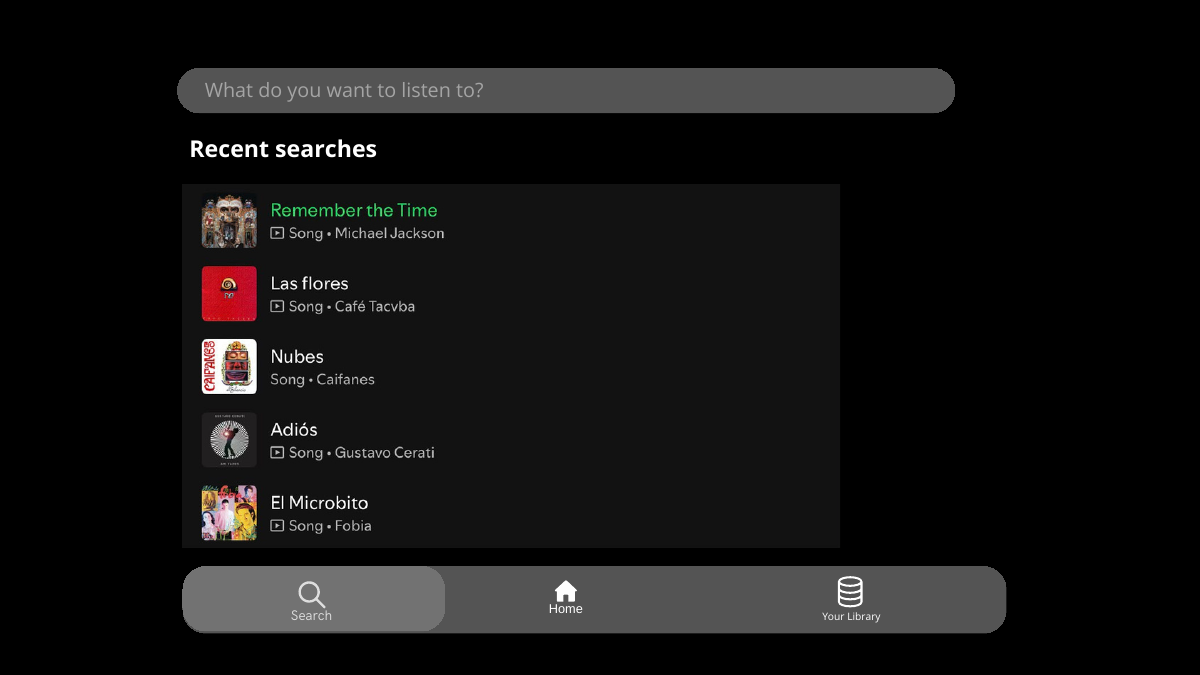
\includegraphics[width=\linewidth]{assets/search.png}\\[-1pt]
{\footnotesize\sffamily Búsqueda e historial: propuesta visual}
\end{minipage}\hfill
\begin{minipage}[t]{0.49\linewidth}\centering
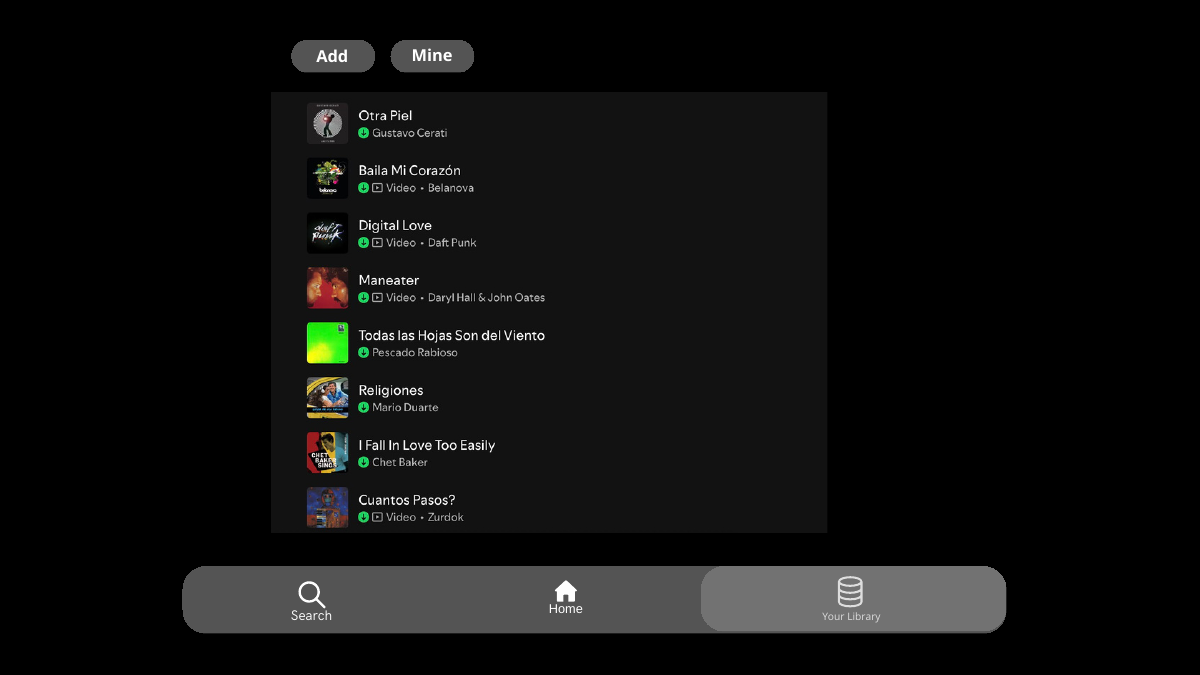
\includegraphics[width=\linewidth]{assets/library.png}\\[-1pt]
{\footnotesize\sffamily Biblioteca con acciones Add y Mine}
\end{minipage}
\caption{Dos bocetos originales de interfaz incorporados como referencia de diseño.}
\end{figure}

Al implementar las vistas se mantuvieron las secciones centrales, la navegación y los formularios. Se replantearon algunas funcionalidades que carecian de soporte en la base: el historial persistente de búsquedas, las carátulas y las fotografias de intérpretes no forman parte del código confirmado; los campos visuales \emph{Add picture} no se conectaron a almacenamiento. Las operaciones \emph{Add} y \emph{Edit}, en cambio, quedaron representadas con controladores especificos, validaciones e IDs reales de SQLite.

\begin{notabox}
\textbf{Tecnologia de interfaz.} Avalonia permite conservar C\# en Linux y separar XAML (composición visual) de C\# (eventos de la vista). En esta aplicación se empleo una organización MVC explicita, aunque Avalonia también facilita patrones MVVM.
\end{notabox}

% ----------------------------------------------------------------------
\section{Integración final entre MusicApp y MusicMiner}
\subsection{Contrato entre procesos}
La integración no consiste en copiar las clases de \R{} al proyecto gráfico. \code{LibraryView} utiliza un selector nativo de directorios y pasa la ruta a \code{MiningController.MineAsync()}. Este controlador verifica directorio, base de datos y ejecutable; construye los argumentos mediante \code{ArgumentList} de \code{ProcessStartInfo}; ejecuta \code{MinerExecutable}; captura \code{stdout} y \code{stderr} en paralelo; espera su finalización sin bloquear directamente la interfaz; y deserializa la última línea JSON que cumpla el formato esperado.

\begin{lstlisting}[style=commands]
MinerExecutable --db "/ruta/rolas.db" --json "/ruta/Musica"
\end{lstlisting}

La respuesta JSON contiene \code{found}, \code{inserted}, \code{duplicates}, \code{skipped}, \code{failed} y \code{reasons}. El controlador de MusicApp exige un código de salida satisfactorio y un JSON interpretable; en caso contrario informa un error. Si el proceso finaliza satisfactoriamente, la vista recarga las canciones desde SQLite y presenta \code{MiningResultView}.

\begin{figure}[H]
\centering
\begin{adjustbox}{max width=\linewidth}
\begin{tikzpicture}[x=1cm,y=1cm]
\foreach \x/\lab in {0/{Usuario},2.9/{LibraryView},5.8/{MiningController},9/{MinerExecutable},12.2/{SQLite}} {
  \node[bluebox,text width=2.35cm,minimum height=0.8cm] (h\x) at (\x,0) {\lab};
  \draw[dashed,grayline] (\x,-0.55) -- (\x,-6.9);
}
\draw[arrow] (0,-1.1) -- node[above,font=\scriptsize]{Mine + carpeta} (2.9,-1.1);
\draw[arrow] (2.9,-2.0) -- node[above,font=\scriptsize]{MineAsync(ruta)} (5.8,-2.0);
\draw[arrow] (5.8,-2.9) -- node[above,font=\scriptsize]{Process / argumentos} (9,-2.9);
\draw[arrow] (9,-3.8) -- node[above,font=\scriptsize]{INSERT / SELECT} (12.2,-3.8);
\draw[dashedarrow] (12.2,-4.5) -- node[above,font=\scriptsize]{resultado de SQL} (9,-4.5);
\draw[dashedarrow] (9,-5.2) -- node[above,font=\scriptsize]{JSON + exit code} (5.8,-5.2);
\draw[dashedarrow] (5.8,-5.9) -- node[above,font=\scriptsize]{MiningReport} (2.9,-5.9);
\draw[arrow] (2.9,-6.55) -- node[above,font=\scriptsize]{Resumen / nueva lista} (0,-6.55);
\end{tikzpicture}
\end{adjustbox}
\caption{Secuencia de ejecucion del minado solicitado desde la interfaz.}
\end{figure}

\subsection{Rutas y despliegue}
Durante el desarrollo aparecio una confusa diferencia entre \emph{carpeta del proyecto} y \emph{nombre del ejecutable}. Aunque el código vive en un directorio \file{MusicMiner}, el archivo compilado es \file{MinerExecutable}; la configuración de MusicApp debe apuntar a esa ruta real, por ejemplo el ejecutable ubicado bajo \file{bin/Debug/net8.0/}. Tambien se distinguio la ruta del directorio que se analiza de la ruta del archivo \file{.db}: ambos programas deben apuntar a la misma base de datos, pues una base bajo \file{~/.local/share/MusicApp/} es diferente de otra creada en el directorio de desarrollo.

La ejecucion final de la integración fue confirmada en una prueba manual: \A{} consiguió iniciar el minero. Sin embargo, la observacion posterior de canciones aparentemente repetidas motivo una nueva revisión del criterio de identidad y del origen de los datos que se mostraban.

% ----------------------------------------------------------------------
\section{Problemas encontrados y ajustes realizados}
\begin{longtable}{@{}p{3.15cm}p{5.35cm}p{6.45cm}@{}}
\caption{Incidencias documentadas, su causa y las medidas de corrección o diagnostico.}\\
\toprule
\textbf{Incidencia} & \textbf{Causa identificada} & \textbf{Respuesta adoptada o pendiente}\\
\midrule
\endfirsthead
\toprule
\textbf{Incidencia} & \textbf{Causa identificada} & \textbf{Respuesta adoptada o pendiente}\\
\midrule
\endhead
Lectura de MP3 sin etiquetas & Archivos descargados desde convertidores no incluian título, álbum u otros metadatos. La prueba con \file{demo.mp3} del curso si devolvio etiquetas. & Se incorporo validación de título, álbum e intérprete; los archivos incompletos se omiten con motivo.\\
\addlinespace
\code{Value must be set} & Un parametro de la consulta de álbum recibia un nombre nulo en \code{GetOrCreateAlbum}. & Se detecto mediante el \emph{stack trace}; la validación previa del minero evita enviar esos archivos a la inserción. La política de etiquetas faltantes puede ampliarse en el futuro.\\
\addlinespace
Consultas SQL incorrectas & Primeras pruebas contenian nombres de parametros repetidos, marcador de género mal escrito y nombre del álbum usado donde correspondia su ID. & Se separaron las resoluciones de intérprete y álbum, se parametrizaron consultas y se gestionaron valores \code{NULL}.\\
\addlinespace
Tres conexiones por inserción & Los métodos auxiliares abrian conexiones independientes. & Se refactorizo la inserción a una sola conexión y transacción compartidas por cancion.\\
\addlinespace
Reimportacion de \file{rolas.sql} & Las tablas e IDs iniciales ya existian en \file{rolas.db}. & Se distinguio creacion del esquema de consulta: usar \code{sqlite3 archivo.db} y \code{SELECT}, no importar el script en cada prueba.\\
\addlinespace
\code{AVLN2000} & Tres vistas XAML usaban \code{ColumnSpacing} de una forma rechazada por la compilación disponible. & Se sustituyó esa separacion visual por margenes entre controles; el proyecto volvió a compilar en el entorno de desarrollo.\\
\addlinespace
\code{CS0050/51/53} & Los tipos \code{Song} expuestos por APIs publicas no tenian accesibilidad equivalente; además, se había colocado el minero bajo el proyecto MusicApp. & Se revisó la visibilidad \code{public} de modelos y se mantuvieron ambos proyectos en carpetas independientes, evitando inclusion accidental de fuentes.\\
\addlinespace
Ejecutable no localizado & Se asumio que el ejecutable se llamaba \file{MusicMiner}. & Se identifico su nombre efectivo \file{MinerExecutable} y se paso su ruta mediante \code{--miner} o \code{MUSICMINER_PATH}.\\
\addlinespace
Canciones repetidas & Se observaron canciones aparentemente duplicadas en la integración; no se confirmó si había igual ruta, rutas distintas o filas duplicadas solo en la vista. & Se propuso verificar \code{GROUP BY path HAVING COUNT(*)>1}, revisar rutas y considerar \code{UNIQUE(path)} tras depurar la base. \textbf{No se da por solucionado.}\\
\bottomrule
\end{longtable}

\subsection{Que ensenaron las pruebas realizadas}
El caso de los archivos provenientes de convertidores evidencio que \emph{tener audio MP3 valido no implica poseer etiquetas ID3 completas}. Por eso las pruebas deben incluir entradas validas, incompletas y corruptas, y no solo el ejemplo \file{demo.mp3}. Asimismo, los errores de compilación mostraron la importancia de compilar cada ejecutable por separado y conservar la division de proyectos. Finalmente, la aparicion de duplicados demostro que el éxito del proceso y la corrección de los registros no son equivalentes: deben verificarse consultas directas a SQLite.

% ----------------------------------------------------------------------
\section{Pruebas recomendadas y estado de validación}
El diseño admite pruebas unitarias de las clases y pruebas de integración sobre una base temporal. La siguiente matriz separa lo \emph{observado durante el desarrollo} de lo que \emph{aun debe verificarse de forma sistematica}.

\begin{table}[H]
\centering\small
\caption{Matriz de verificacion y evidencia disponible.}
\begin{tabularx}{\linewidth}{@{}p{4.3cm}p{2.65cm}X@{}}
\toprule
\textbf{Prueba} & \textbf{Estado} & \textbf{Evidencia o criterio de aceptacion}\\
\midrule
Compilar MusicApp & Reportada como exitosa & Los errores XAML previos dejaron de presentarse.\\
Invocar MusicMiner desde MusicApp & Reportada como exitosa & El minero se ejecuta como proceso externo.\\
Leer \file{demo.mp3} & Observada & Etiquetas de ejemplo (título T, álbum L, año 1950, género Jazz) fueron leidas.\\
MP3 sin metadatos & Observada & Cinco archivos fueron omitidos tras el diagnostico; revisar motivos.\\
ID3v2.2, v2.3 y v2.4 & Pendiente de bateria formal & Usar archivos controlados de cada variante y verificar etiquetas.\\
Insertar dos veces la misma ruta & Por verificar & La cantidad de filas para esa ruta debe permanecer en 1.\\
Controlar copias en rutas distintas & Pendiente de definir & Acordar si son dos archivos validos o duplicados de contenido.\\
Fallos de inserción y transacciones & Pendiente & Ninguna inserción parcial de la misma cancion debe permanecer.\\
Alta y edición desde formularios & Pendiente de bateria formal & Los cambios deben reflejarse en \code{SELECT} por ID.\\
Consistencia de estadisticas JSON & Pendiente de ajuste & \code{inserted}, \code{duplicates} y \code{failed} deben ser contadores reales.\\
\bottomrule
\end{tabularx}
\end{table}

\subsection{Consultas de comprobacion}
Las siguientes consultas pueden ejecutarse sobre \textbf{una copia de la base de datos} de pruebas. Sirven para revisar resultados sin depender exclusivamente de lo que muestre la interfaz.
\begin{lstlisting}[style=commands]
SELECT id_rola, title, path FROM rolas ORDER BY id_rola DESC;
SELECT path, COUNT(*) AS repeticiones
FROM rolas GROUP BY path HAVING COUNT(*) > 1;
PRAGMA foreign_key_check;
\end{lstlisting}

% ----------------------------------------------------------------------
\section{Limitaciones y líneas de mejora}
\begin{enumerate}
\item \textbf{Definir identidad de canciones.} La comprobacion por ruta exacta no detecta copias identicas en otras carpetas y no basta contra inserciones concurrentes; evaluar normalizacion de rutas, restricciones unicas o hashes, conforme a los requisitos.
\item \textbf{Corregir estadisticas.} Devolver no solo el ID de \code{GetOrCreateSong}, sino también si se inserto o se reutilizo. Separar \code{Skipped} por metadatos insuficientes de \code{Failed} por excepción.
\item \textbf{Corregir el estado de salida.} Un fallo general atrapado dentro de \code{Miner.Mina} debe reflejarse en el estado devuelto al proceso solicitante.
\item \textbf{Alinear criterios de álbum.} El minero usa nombre y ruta de carpeta, mientras que la inserción manual de MusicApp busca por nombre; definir una identidad consistente para evitar álbumes ambiguos.
\item \textbf{Reforzar las relaciones de personas y grupos.} El esquema recibido no conecta explicitamente personas con intérpretes; ampliar la base o formalizar la convención para impedir colisiones.
\item \textbf{Agregar campos gráficos futuros.} Para carátulas, fotos de artistas e historial de búsquedas sería necesario decidir almacenamiento y reglas de actualizacion.
\item \textbf{Completar la cobertura de etiquetas.} Validar ID3v2.2/2.3/2.4, varios artistas, varios géneros, años ausentes, archivos corruptos y caracteres Unicode.
\item \textbf{Verificar el despliegue.} Resolver automáticamente la ruta de \file{MinerExecutable} en compilaciones distribuidas y documentar las opciones \code{--miner} y \code{--db}.
\end{enumerate}

% ----------------------------------------------------------------------
\section{Conclusiones}
El proyecto fue evolucionando desde una tarea aparentemente simple ---encontrar MP3 y guardarlos en una tabla--- hasta una arquitectura de dos programas que comparte una base relacional. La dificultad principal no estuvo en la enumeracion de archivos, que ya resuelve .NET, sino en definir \textbf{limites de responsabilidad}: que hace cada clase, como se transportan los metadatos, como se resuelven las claves foraneas, como se distinguen errores y omisiones y como se comunica un ejecutable con otro.

Las decisiones de diseño evolucionaron conforme aparecieron casos reales. Se mantuvo la division entre \code{Search}, \code{Analyze} y \code{AddDataBase}; se introdujo un objeto \code{Song} específico para etiquetas; se sustituyeron conexiones repetidas por una transacción compartida por cancion; se paso de un mensaje único a resultados estructurados; y se reorganizo MusicApp para evitar un MVC anidado. La integración mediante argumentos, JSON y \code{ProcessStartInfo} permitió preservar la independencia del minero.

El estado documentado confirma una \textbf{integración funcional básica} y una interfaz capaz de operar con SQLite, pero también muestra asuntos por concluir: identidad de canciones, contadores confiables, manejo explicito de fallos generales y cobertura sistematica de versiones ID3. Esta distincion entre lo implementado y lo pendiente es parte de una evaluación técnica rigurosa del proyecto.

% ----------------------------------------------------------------------
\appendix
\section{Inventario de fuentes analizadas}
\begin{tabularx}{\linewidth}{@{}p{3.0cm}X@{}}
\toprule
\textbf{Componente} & \textbf{Archivos utilizados para analizar su funcionamiento}\\
\midrule
MusicMiner & \file{Program.cs}, \file{Miner.cs}, \file{Search.cs}, \file{Analyze.cs}, \file{Song.cs}, \file{AddDataBase.cs}, \file{MiningResult.cs}, \file{Message.cs}, \file{MinerExecutable.csproj}, \file{README_MusicMiner.md}.\\
MusicApp & \file{AppConfig.cs}, \file{Program.cs}, \file{MusicApp.csproj}, \file{Model/Find.cs}, \file{Model/LibraryEditor.cs}, \file{Model/Database.cs}, \file{Controller/Finder.cs}, \file{Controller/LibraryController.cs}, \file{Controller/MiningController.cs}, \file{Controller/Result.cs}, \file{Controller/DbAccess.cs}, y vistas Avalonia.\\
Esquema y bocetos & \file{rolas.sql} e \file{InterfazApp.pdf}.\\
\bottomrule
\end{tabularx}

\section{Arbol conceptual del repositorio}
\begin{lstlisting}[style=commands]
proyecto2/
|-- MusicApp/
|   |-- Model/         Song, Artist, Album, Find, LibraryEditor...
|   |-- Controller/    Finder, LibraryController, MiningController...
|   |-- View/          XAML, formularios, biblioteca y resultados
|   `-- MusicApp.csproj
|-- MusicMiner/
|   |-- model/         Song, Search, Analyze, AddDataBase, MiningResult
|   |-- controller/    Miner
|   |-- view/          Message
|   `-- MinerExecutable.csproj
`-- rolas.sql          Script de esquema; no es el archivo .db
\end{lstlisting}

\section{Comandos de uso y depuracion}
\begin{lstlisting}[style=commands]
# Compilar proyectos de manera independiente
cd MusicMiner && dotnet build
cd ../MusicApp && dotnet build

# Ejecutar minero desde su directorio
./bin/Debug/net8.0/MinerExecutable \
  --db "/ruta/a/rolas.db" --json "/ruta/a/mp3"

# Iniciar MusicApp indicando la ubicacion real del minero
dotnet run -- \
  --db "/ruta/a/rolas.db" \
  --miner "/ruta/a/MinerExecutable"

# Consultar la base real (sin reimportar rolas.sql)
sqlite3 "/ruta/a/rolas.db"
\end{lstlisting}


\section{Criterios de aceptación para la demostración}
Para presentar el proyecto, se propone realizar la siguiente secuencia sobre una copia del archivo \file{.db}, conservando evidencia de la terminal y de los registros resultantes:
\begin{enumerate}
\item Iniciar \A{} con las opciones \code{--db} y \code{--miner} apuntando a rutas existentes.
\item Buscar por nombre una canción, un álbum y un intérprete; verificar una búsqueda sin coincidencias.
\item Agregar y editar un registro desde los formularios y comprobar su ID mediante una consulta \code{SELECT}.
\item Seleccionar una carpeta con MP3 etiquetados y ejecutar \code{Mine}; verificar que la interfaz no se bloquee y que presente el resultado.
\item Repetir el minado sobre los mismos archivos; revisar tanto los contadores como las filas reales en SQLite para detectar posibles duplicaciones.
\item Probar un archivo sin etiquetas completas y otro corrupto; comprobar que ambos produzcan un motivo y no detengan innecesariamente el resto del lote.
\end{enumerate}
\begin{notabox}
Los resultados de esta demostración deben interpretarse junto con las limitaciones del código actual. En particular, un valor alto de \code{inserted} no garantiza que se hayan creado tantas filas nuevas y \code{duplicates=0} no es todavía una medida real.
\end{notabox}

\vfill
\begin{center}
{\color{green}\rule{0.28\linewidth}{1.3pt}}\\[6pt]
{\footnotesize\sffamily\color{muted}Fin del reporte técnico}
\end{center}
\end{document}
